
\documentclass[9pt]{beamer}
%\makeatletter
%\def\beamer@calltheme#1#2#3{%
%	\def\beamer@themelist{#2}
%	\@for\beamer@themename:=\beamer@themelist\do
%	{\usepackage[{#1}]{\beamer@themelocation/#3\beamer@themename}}}
%
%\def\usefolder#1{
%	\def\beamer@themelocation{#1}
%}
%\def\beamer@themelocation{}

%\usefolder{../config}

\usetheme[
block=fill,
titleformat=regular,
progressbar=frametitle
]{metropolis}
%\metroset[everytitleformat=regular] % regular, lowercase, uppercase ]
%\metroset[inner/block=fill]

%\setbeameroption{show notes} 
\usepackage{booktabs}
\usepackage[scale=2]{ccicons}

\usepackage{pgfplots}
\usepgfplotslibrary{dateplot}


%\ Hrvatski znakovi
\usepackage[utf8]{inputenc}
\usepackage[T1]{fontenc}
\usepackage[croatian]{babel}
\usepackage{todonotes}
\usepackage{amsmath}
\usepackage{amsfonts}
\selectlanguage{croatian} % american ngerman
\usepackage{todonotes}

% Koristenje Latin modern fonta
% Bez toga na nekim racunalima baca
% err: Font <taj i taj> at <mala velicina, npr4.0pt> not loadable: Metric (TFM) file not found. \end{frame}
\usepackage{lmodern}


\definecolor{RoyalBlue}{cmyk}{1, 0.50, 0, 0}
%\usepackage{natbib}
%\usepackage{bibentry}
\usepackage{scrextend}
\usepackage{hyperref}
%\usepackage[pdfa=true]{hyperref}
\hypersetup{%
    %draft, % = no hyperlinking at all (useful in b/w printouts)
    %colorlinks=true, 
    linktocpage=true, pdfstartpage=3, pdfstartview=FitV,%
    % uncomment the following line if you want to have black links (e.g., for printing)
    %colorlinks=false, linktocpage=false, pdfborder={0 0 0}, pdfstartpage=3, pdfstartview=FitV,% 
    breaklinks=true, pdfpagemode=UseNone, pageanchor=true, pdfpagemode=UseOutlines,%
    plainpages=false, bookmarksnumbered, bookmarksopen=true, bookmarksopenlevel=1,%
    hypertexnames=true, pdfhighlight=/O,%nesting=true,%frenchlinks,%
    %urlcolor=webbrown, linkcolor=RoyalBlue, citecolor=webgreen, %pagecolor=RoyalBlue,%
    %urlcolor=Blue, linkcolor=Blue, citecolor=Red, %pagecolor=Black,%
    %pdftitle={\myTitle},%
    %pdfauthor={\textcopyright\ \myName, \myUni, \myFaculty},%
    pdfsubject={},%
    pdfkeywords={},%
    pdfcreator={pdfLaTeX},%
    pdfproducer={LaTeX with hyperref and classicthesis}, %
    unicode = true 
} 

%\usepackage[pdftex]{graphicx}
% declare the path(s) where your graphic files are
\graphicspath{{./}{./figures/}}


\newcommand{\executeiffilenewer}[3]{%
	\ifnum\pdfstrcmp{\pdffilemoddate{#1}}%
	{\pdffilemoddate{#2}}>0%
	{\immediate\write18{#3}}\fi%
}
\newcommand{\includesvg}[1]{%
	\executeiffilenewer{#1.svg}{#1.pdf}%
	{inkscape -z -C --file=#1.svg %
		--export-pdf=#1.pdf --export-latex}%
	\input{#1.pdf_tex}%
}


% http://tex.stackexchange.com/questions/83882/how-to-highlight-python-syntax-in-latex-listings-lstinputlistings-command

\usepackage{listings}
\usepackage{color}
\usepackage[semibold]{sourcecodepro}

% Default fixed font does not support bold face
\DeclareFixedFont{\ttb}{T1}{txtt}{bx}{n}{12} % for bold
\DeclareFixedFont{\ttm}{T1}{txtt}{m}{n}{12}  % for normal
% Custom colors
\definecolor{deepblue}{rgb}{0,0,0.5}
\definecolor{deepred}{rgb}{0.6,0,0}
\definecolor{deepgreen}{rgb}{0,0.5,0}


% Python style for highlighting
\newcommand\pythonstyle{\lstset{
		language=Python,
		basicstyle=\small\ttfamily,
		otherkeywords={self},             % Add keywords here
		keywordstyle=\small\ttfamily\color{deepblue},
		emph={MyClass,__init__},          % Custom highlighting
		emphstyle=\small\ttfamily\color{deepred},    % Custom highlighting style
		stringstyle=\color{deepgreen},
		frame=tb,                         % Any extra options here
		showstringspaces=false            % 
	}}
	
	
	% Python environment
	\lstnewenvironment{python}[1][]
	{
		\pythonstyle
		\lstset{#1}
	}
	{}
	
	% Python for external files
	\newcommand\pythonexternal[2][]{{
			\pythonstyle
			\lstinputlisting[#1]{#2}}}
	
	% Python for inline
	\newcommand\pythoninline[1]{{\pythonstyle\lstinline!#1!}}
%\documentclass[ucs]{beamer}
%\usetheme[menuwidth={0.3\paperwidth}]{erlangen}
%\setbeamercovered{transparent=20} 

\usepackage{amsmath,amsfonts,amsthm,amssymb}
\usepackage{setspace}
\usepackage{Tabbing}
\usepackage{fancyhdr}
\usepackage{lastpage}
\usepackage{extramarks}
\usepackage{chngpage}
\usepackage{soul,color}
\usepackage{graphicx,float,wrapfig}
\usepackage{xcolor}
\usepackage[normalem]{ulem}
\usepackage{mathtools}
\usepackage{cancel}

\definecolor{erlangenlyellow}{RGB}{123, 25, 121}
%\usepackage[utf8x]{inputenc}
%\usepackage{default}
%\usepackage[T1]{fontenc}

\usepackage{verbatim}
\usepackage{listings}
\usepackage{algorithm2e}


\usepackage{subcaption}
\usepackage{lmodern}

\title{Ray tracing i prostor}

\subtitle{Podnaslov}
\institute{Računalna grafika}

% Delete this, if you do not want the table of contents to pop up at
% the beginning of each subsection:
%\AtBeginSubsection[]
%{
%  \begin{frame}<beamer>{Outline}
%    \tableofcontents[currentsection,currentsubsection]
%  \end{frame}
%}
%
%\AtBeginSection[]
%{
%  \begin{frame}<beamer>{Outline}
%    \tableofcontents[currentsection]
%  \end{frame}
%}

\begin{document}
\begin{frame}
 \titlepage
\end{frame}

\begin{frame}{Sadržaj}
  \tableofcontents
  % You might wish to add the option [pausesections]
\end{frame}

%
%\begin{frame}{Render jednadžba}
%	\begin{align*}
%	L_o(X, \hat{\omega}_o) = L_e(X, \hat{\omega}_e) +
%	 \int_{S^2}  L_i(X, \hat{\omega}_i) f_X(\hat{\omega}_i), \hat{\omega}_o)) \left|\hat{\omega}_i\cdot \hat{n}\right| 
%	 \mathrm{d} \hat{\omega}_i
%	\end{align*}
%	\begin{itemize}
%		\item $X$: točka u sceni
%		\item $\hat{\omega}_o$: izlazni smjer(\textit{outgoing dir}), smjer prema očištu
%		\item $\hat{\omega}_i$: dolazni, ulazni smjer(\textit{incoming dir}), smjer svjetla na točku $X$ 
%    	\item $\hat{n}$: normala površine
%		\item $S^2$: svi dolazni, ulazni smjerovi(\textit{incoming directions})
%	\end{itemize}
%\end{frame}
%
%\begin{frame}{Render jednadžba}
%	\begin{align*}
%	L_o(X, \hat{\omega}_o) = L_e(X, \hat{\omega}_e) +
%	\int_{S^2}  L_i(X, \hat{\omega}_i) f_X(\hat{\omega}_i), \hat{\omega}_o)) \left|\hat{\omega}_i\cdot \hat{n}\right| 
%	\mathrm{d} \hat{\omega}_i
%	\end{align*}
%	\begin{itemize}
%		\item $L_o(X, \hat{\omega}_o)$: Izlazno svjetlo - Kakav je rezultirajući intenzitet svjetla za zadanu točku i smjer?
%		\item $L_e(X, \hat{\omega}_e)$: Emitirano svjetlo - Kakav je intenzitet svjetla koji emitira zadana točka za zadani smjer? - Recimo izvor svjetla
%		\item $L_i(X, \hat{\omega}_i)$: Dolazno, ulazno svjetlo - za zadanu točku koji intenzitet svjetla vidim za zadani smjer?
%		\item $f_X(\hat{\omega}_i), \hat{\omega}_o))$: Materijal - za zadani ulazni i izlazni smjer, koji intenzitet svjetla ide u izlaznom smjeru?
%		\item $\left|\hat{\omega}_i\cdot \hat{n}\right|$: Lambert - geometrijski izraz, recimo, difuzni 
%	\end{itemize}
%\end{frame}
%
%\begin{frame}{Render jednadžba}
%	\begin{align*}
%	L_o(X, \hat{\omega}_o) = L_e(X, \hat{\omega}_e) +
%	\int_{S^2}  L_i(X, \hat{\omega}_i) f_X(\hat{\omega}_i), \hat{\omega}_o)) \left|\hat{\omega}_i\cdot \hat{n}\right| 
%	\mathrm{d} \hat{\omega}_i
%	\end{align*}
%	\begin{itemize}
%		\item $S^2$: svi dolazni, ulazni smjerovi(\textit{incoming directions})
%		\item $\mathrm{d} \hat{\omega}_i$
%	\end{itemize}
%Pure Path tracing: zbrojimo sva svjetla iz svih smjerova
%\end{frame}



\section{BVH}

\begin{frame}{Ideja}
	\begin{itemize}
		\item Nije potrebno računati presjecište s primitivom ako zraka \textit{sigurno} ne siječe primitiv
		\item Npr. zraka sigurno nema sjecište ako nema presjecište s omeđujućim kvadrom (\textit{bounding box})
	\end{itemize}
\begin{center}
	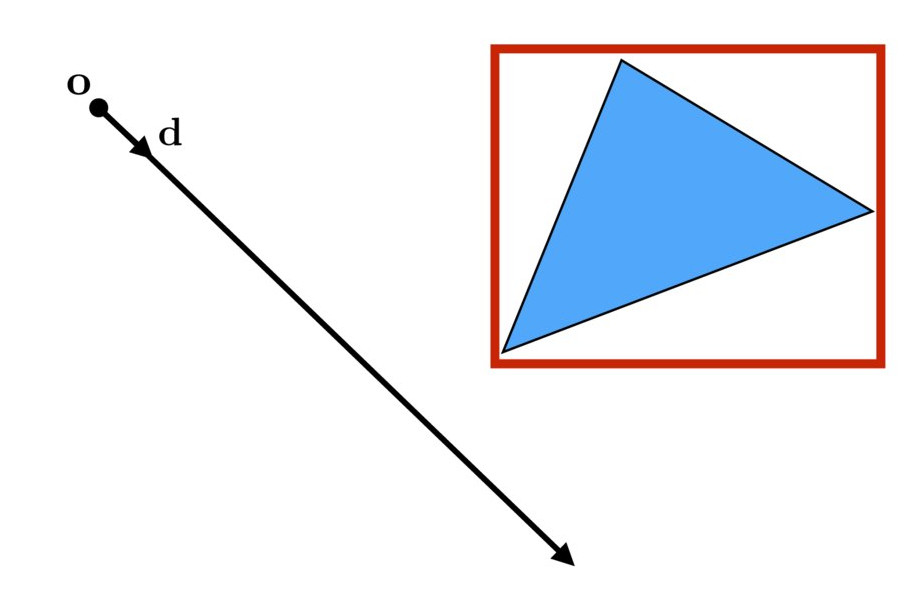
\includegraphics[width=0.5\textwidth]{slike/slide_005.jpg}
\end{center}
\end{frame}

\begin{frame}{Ideja}
	\begin{columns}
		\begin{column}{0.5\textwidth}
				\begin{center}
				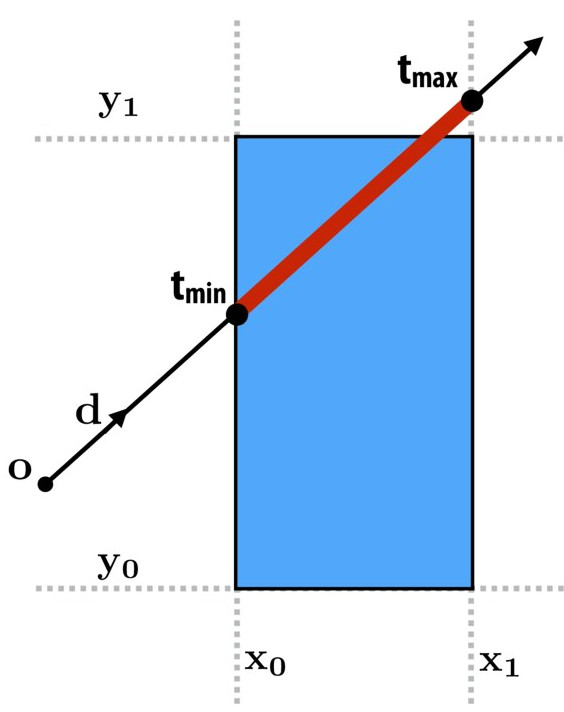
\includegraphics[width=0.8\textwidth]{slike/slide_006.jpg}
			\end{center}
		\end{column}
	\begin{column}{0.5\textwidth}
		\begin{align*}
		\mathbf{P}(t) = \mathbf{o} + t\mathbf{d}
		\end{align*}
		\begin{align*}
		t0 &= \frac{x_0 - \mathbf{o}_x}{\mathbf{d}_x} \\
		t1 &= \frac{x_1 - \mathbf{o}_x}{\mathbf{d}_x}
		\end{align*}
		Jednostavnije, može se izračunati:
		\begin{align*}
		a = \frac{1}{\mathbf{d}_x} \qquad b = -\frac{\mathbf{o}_x}{\mathbf{d}_x}
		\end{align*}
		Sada je
		\begin{align*}
		t_0 = a x_0 + b \qquad t_1 = a x_1 + b
		\end{align*}
	\end{column}
	\end{columns}
\end{frame}


\begin{frame}{Ideja}
	\begin{itemize}
		\item Izračunati presjecišta sa svim ravninama
		\item Kako znamo je li zraka \textit{promašila} kvadar?
	\end{itemize}
	\begin{center}
		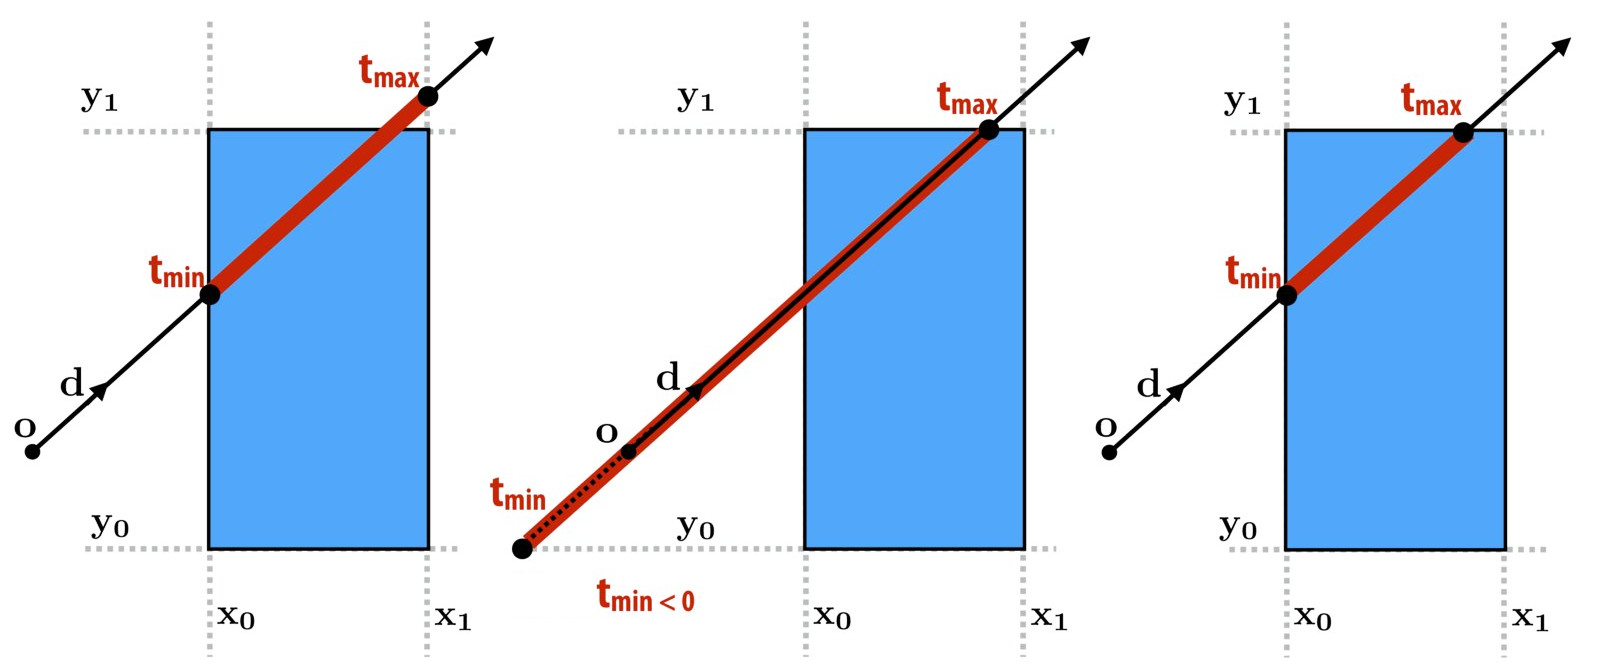
\includegraphics[width=0.8\textwidth]{slike/slide_007.jpg}
	\end{center}
\begin{center}
	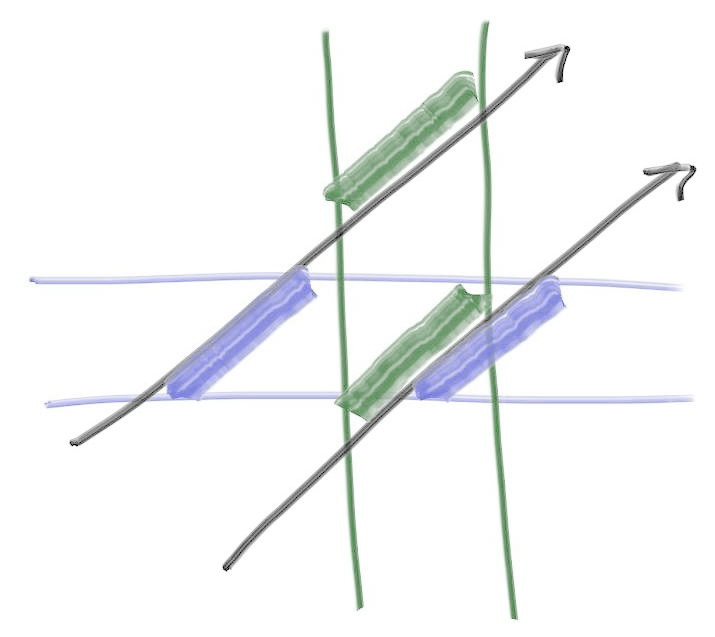
\includegraphics[width=0.3\textwidth]{slike/fig.rstio.jpg}
\end{center}
\end{frame}


\begin{frame}{Problem}
	\begin{columns}
		\begin{column}{0.5\textwidth}
			\begin{algorithm}[H]
				\SetAlgoLined
%				\KwResult{Write here the result }
					p\_closest = nullpltr\;
					t\_closest = inf\;
				\For{each primitive p u sceni}{
					\If{!p.bbox.intersect(r)}{
						continue\;
					}
					t = p.intersect(r)\;
					\If{t >0 \&\& t < t\_closest}{
						t\_closest = t\;
						p\_closest = p\;
					}
				}
			\end{algorithm}
		I dalje smo na \textit{O(N)}!
		\end{column}
		\begin{column}{0.5\textwidth}
			\begin{center}
				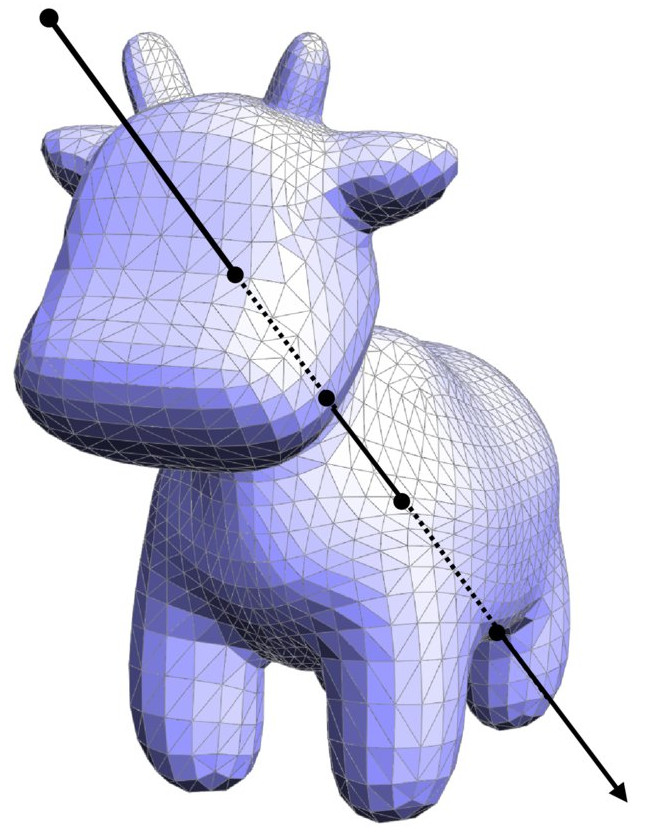
\includegraphics[width=0.8\textwidth]{slike/slide_008.jpg}
			\end{center}
		\end{column}
	\end{columns}
\end{frame}

\begin{frame}{Jednostavniji problem}
	\begin{itemize}
		\item Zadana lista brojeva \textbf{S}
		\item Za zadani broj, npr. $k=18$, naći najbliži element iz \textbf{S}
	\end{itemize}
	\begin{center}
		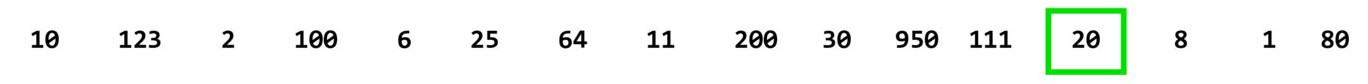
\includegraphics[width=0.8\textwidth]{slike/slide_011_a.jpg}
	\end{center}
	\begin{itemize}
		\item Grozno
		\item Sortirajmo elemente
	\end{itemize}
	\begin{center}
		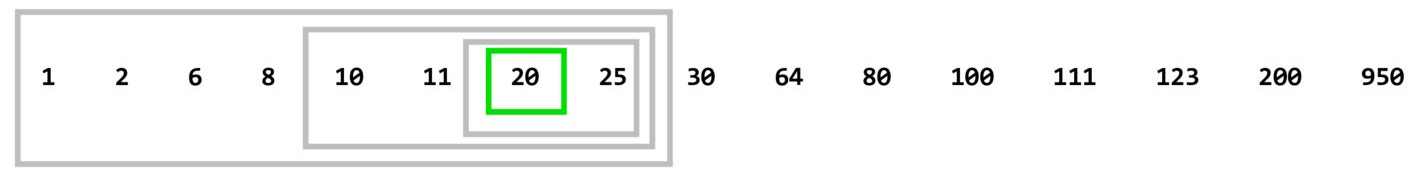
\includegraphics[width=0.8\textwidth]{slike/slide_011_b.jpg}
	\end{center}
	\begin{itemize}
		\item Kompleksnost algoritma za jedan opit: $O(n \log n)$
		\item Puno upita: $O(\log n)$
	\end{itemize}
\end{frame}

\begin{frame}{Jednostavni slučaj}
	\begin{center}
		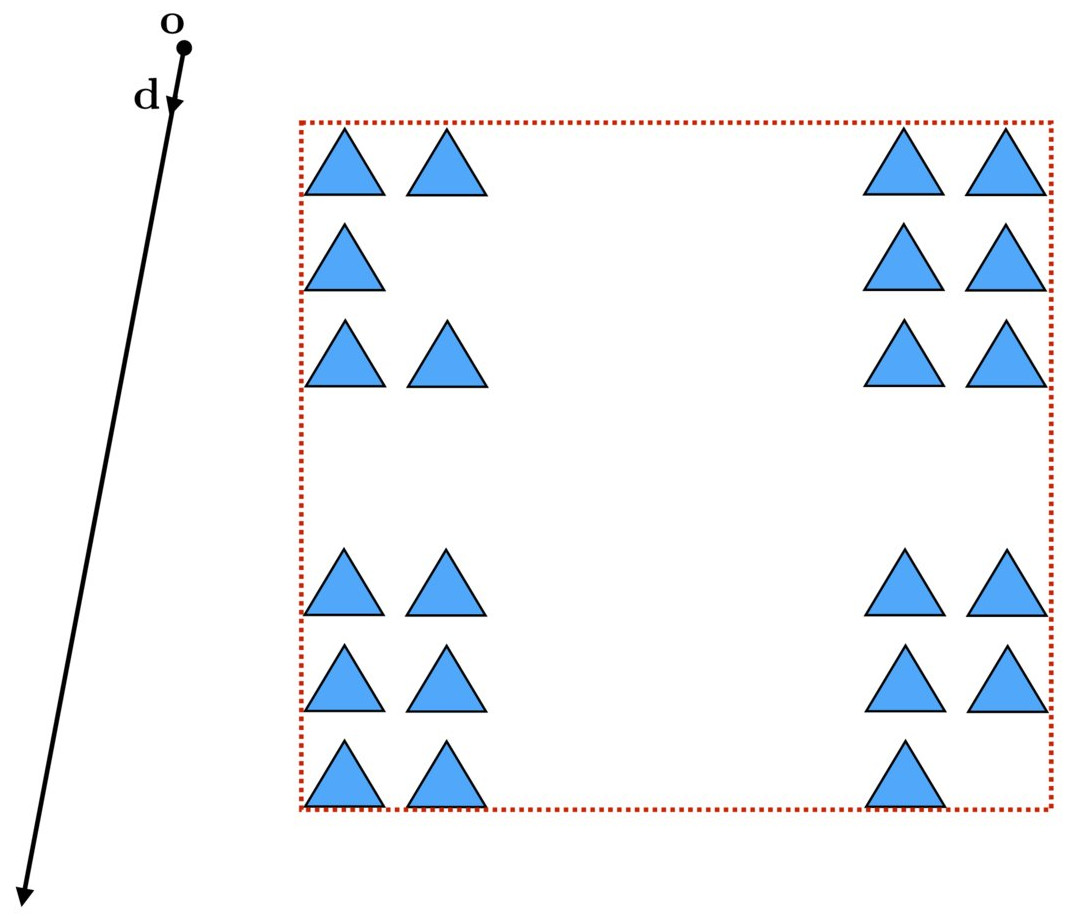
\includegraphics[width=0.5\textwidth]{slike/slide_013.jpg}
	\end{center}
	\begin{itemize}
		\item Zraka ne siječe omeđujući kvadar
		\item preprocess: $O(N)$
		\item ray-box test: $O(1)$
		\item puno ray-box testova: $O(1)$
	\end{itemize}
\end{frame}

\begin{frame}{Jednostavni slučaj}
	\begin{center}
		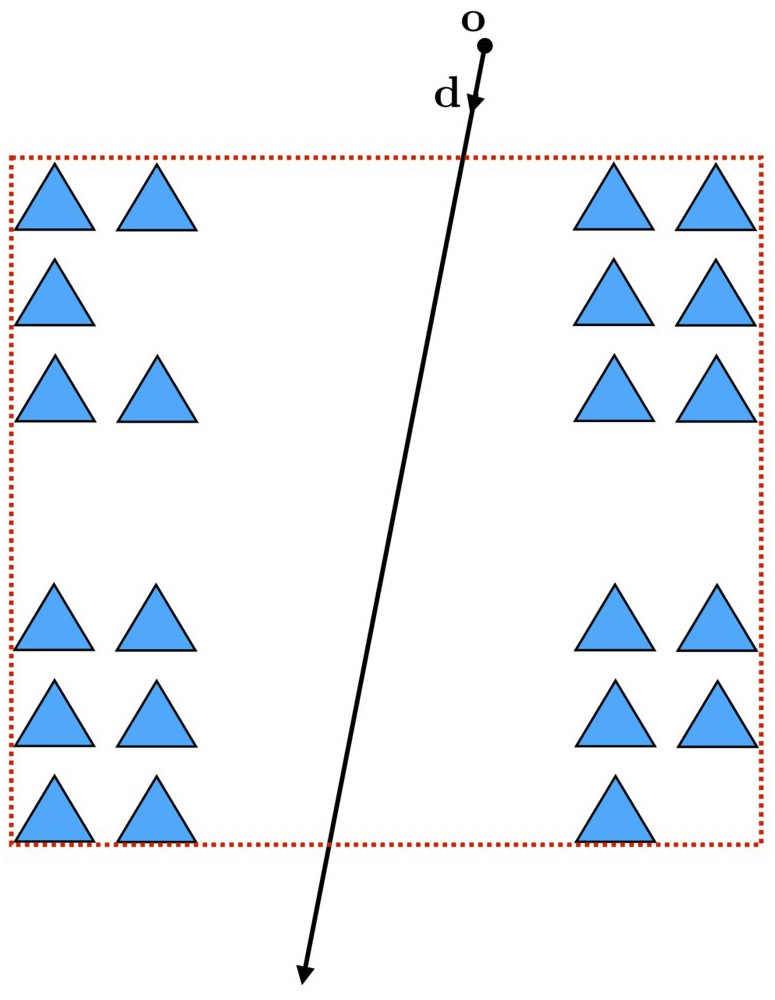
\includegraphics[width=0.3\textwidth]{slike/slide_014.jpg}
	\end{center}
	\begin{itemize}
		\item Zraka ne siječe omeđujući kvadar
		\item preprocess: $O(1)$
		\item ray-box test: $O(1)$
		\item test za primitive: $O(N)$
		\item puno testova: $O(N)$
	\end{itemize}
I dalje nije bolje od početnog algoritma
\end{frame}

\begin{frame}{BVH}
	\begin{center}
		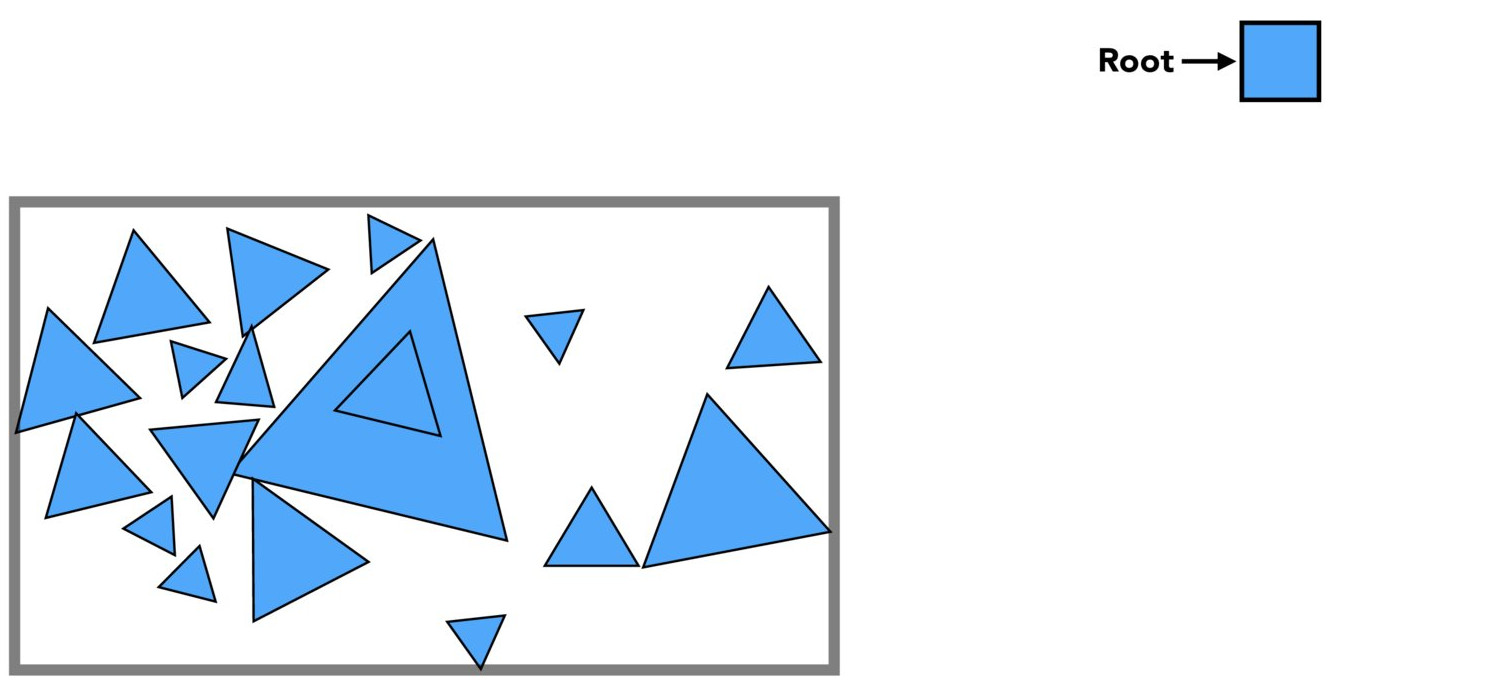
\includegraphics[width=0.8\textwidth]{slike/slide_016.jpg}
	\end{center}
\end{frame}
\begin{frame}{BVH}
	\begin{itemize}
		\item Podijelimo primitive na dva \textit{disjunktna} skupa
		\item Skupovi se mogu i preklapati
	\end{itemize}
	\begin{center}
		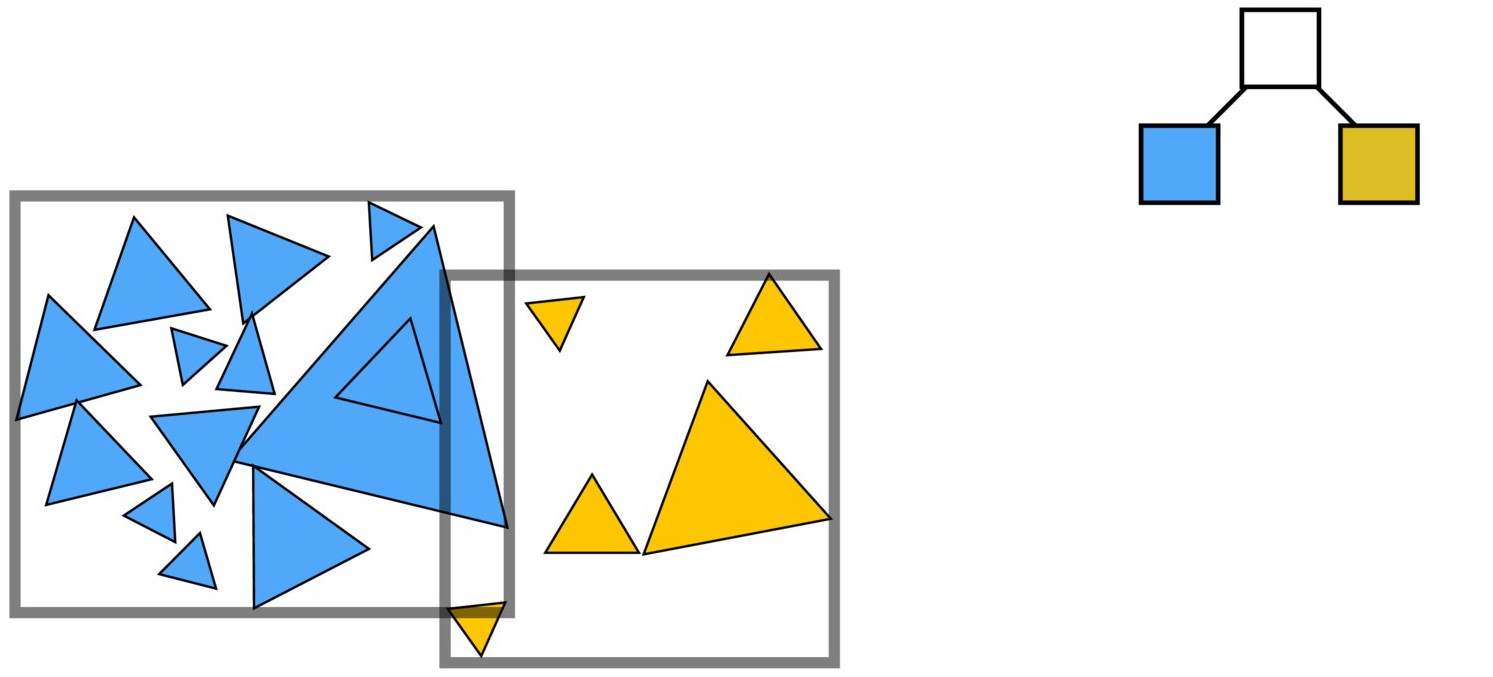
\includegraphics[width=0.8\textwidth]{slike/slide_017.jpg}
	\end{center}
\end{frame}
\begin{frame}{BVH}
	\begin{center}
		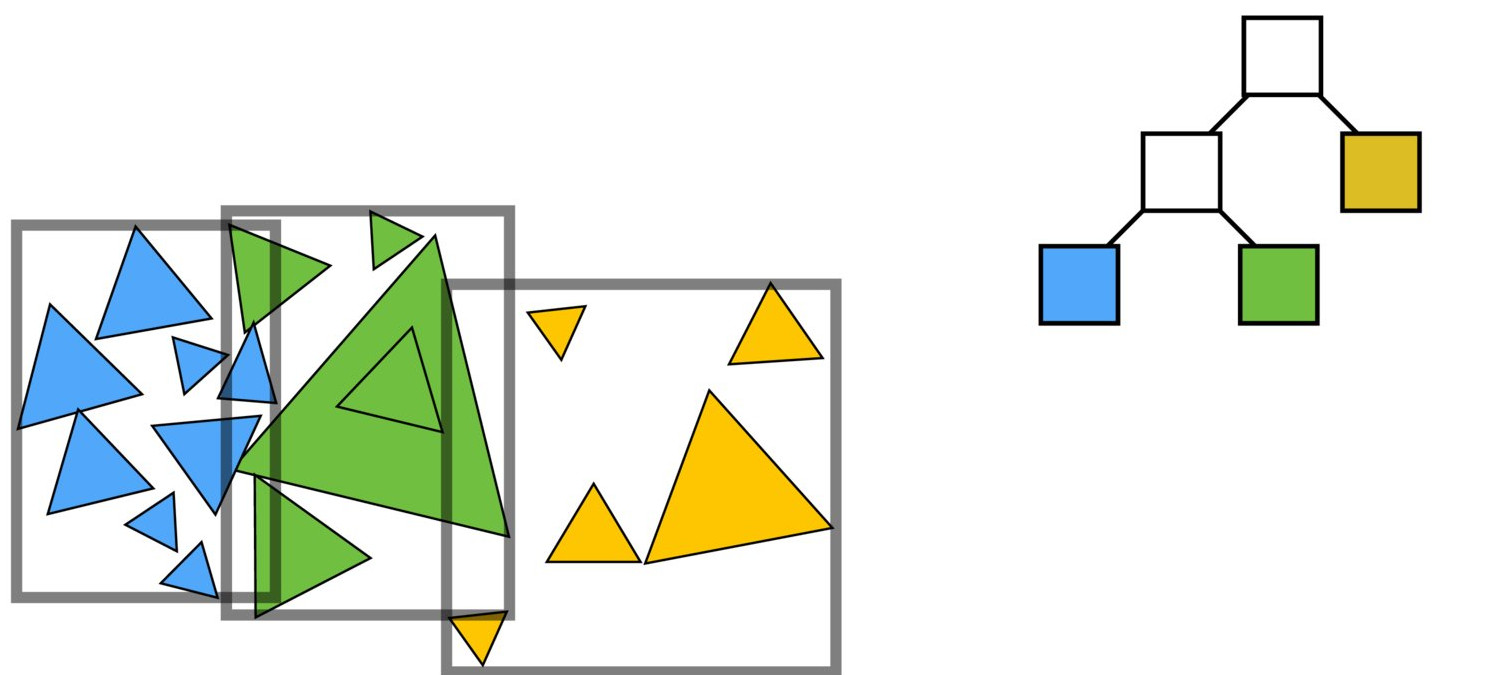
\includegraphics[width=0.8\textwidth]{slike/slide_018.jpg}
	\end{center}
\end{frame}
\begin{frame}{BVH}
	\begin{itemize}
		\item Leaf node (listovi): Sadrže mali broj primitiva
		\item \textit{Interior nodes} Unutrašnji čvorovi
		\begin{itemize}
			\item Proxy za \textit{veliki} podskup primitiva
			\item Sprema omeđujući kvadar za sve primitive tog podstabla
		\end{itemize}
	\end{itemize}
	\begin{center}
		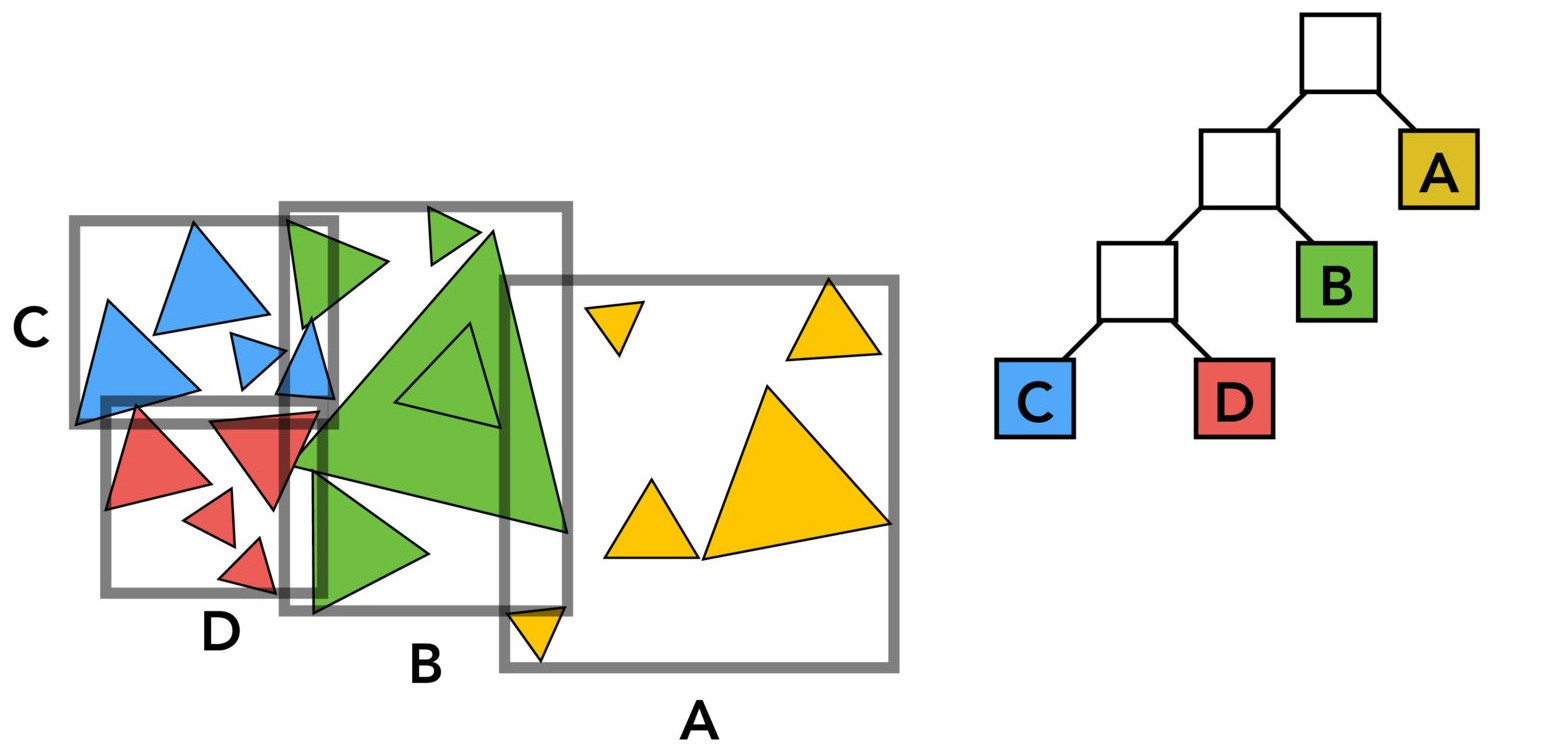
\includegraphics[width=0.8\textwidth]{slike/slide_019.jpg}
	\end{center}
\end{frame}

\begin{frame}{BVH}
	\begin{itemize}
		\item Podjela nije jedinstvena
		\item Koje 
	\end{itemize}
	\begin{center}
		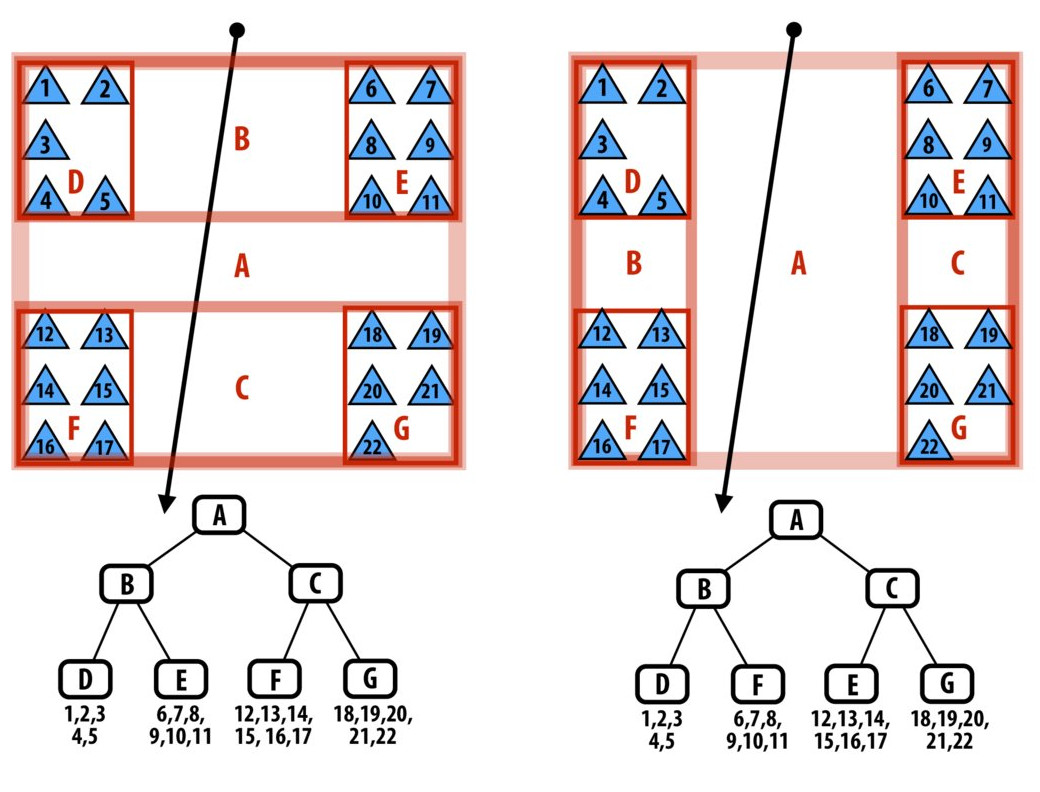
\includegraphics[width=0.8\textwidth]{slike/slide_020.jpg}
	\end{center}
\end{frame}

\begin{frame}{BVH}
	\begin{itemize}
		\item Kako podijeliti primitive u dvije grupe?
	\end{itemize}
	\begin{center}
		
\includegraphics[width=0.8\textwidth]{slike/slide_026.jpg}
	\end{center}
\end{frame}

\begin{frame}{BVH}
	\begin{itemize}
		\item A sada?
	\end{itemize}
	\begin{center}
		
\includegraphics[width=0.8\textwidth]{slike/slide_027.jpg}
	\end{center}
\end{frame}

\begin{frame}{BVH}
	\begin{itemize}
		\item Podjela u dvije grupe s približno istim brojem primitiva
	\end{itemize}
	\begin{center}
		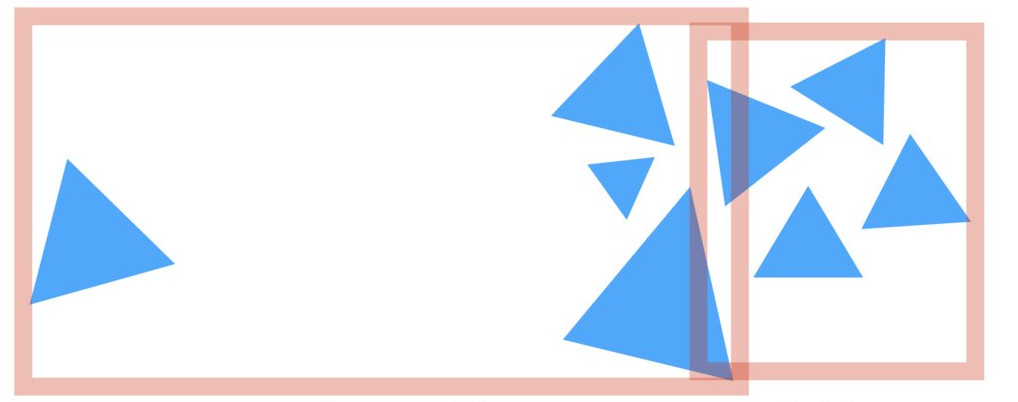
\includegraphics[width=0.6\textwidth]{slike/slide_028_a.jpg}
	\end{center}
	\begin{itemize}
		\item Bolje rješenje:
		\item Želimo male omeđujuće kvadre (minimizirati preklapanje), izbjegavati omeđujuće kvadre koji imaju puno praznog prostora	
	\end{itemize}
	\begin{center}
		
\includegraphics[width=0.6\textwidth]{slike/slide_028_b.jpg}
	\end{center}
\end{frame}

\begin{frame}{BVH, što želimo postići?}
	\begin{itemize}
		\item Kvalitetna podjela minimizira proračunski napor (\textit{cost})nalaženja najbližeg presjecišta zrake sa primitivima u čvoru
	\end{itemize}
Ako je čvor \textit{leaf}:
	\begin{align*}
		C &= \sum_{i=1}^{N} C_{isect}(i) \\
		  &= N C_{isect}
	\end{align*}
	\begin{itemize}
		\item $C_{isect}(i)$:  proračunski napor najbližeg presjecišta zrake s primitivom $i$. 
		\item  $N C_{isect}$ : Ako svi primitivi imaju isti $C_{isect}$
	\end{itemize}
\end{frame}

\begin{frame}{BVH, kreiranje particije}
	\begin{itemize}
		\item Ukupni proračunski napor (\textit{cost})nalaženja najbližeg presjecišta zrake sa primitivima u čvorovima $A$ i $B$
	\end{itemize}
	\begin{align*}
		C = C_{trav} + p_AC_A + p_BC_B
	\end{align*}
	\begin{itemize}
		\item $C_{trav}$: traversal, proračunski napor: (load + provjera siječe li zraka bbox ili ne)
		\item $C_{A}$ i $C_{B}$:  proračunski napor najbližeg presjecišta zrake s čvorovima $A$ i $B$. 
		\item $p_{A}$ i $p_{B}$:  vjerojatnost kojom će zraka presjeći omeđujući kvadar čvorova $A$ i $B$. 
	\end{itemize}
	\begin{align*}
	C = C_{trav} + p_AN_A C_{isect} + p_BN_B C_{isect}
	\end{align*}
	Kako odrediti vjerojatnost?
\end{frame}

\begin{frame}{BVH, određivanje vjerojatnosti}
	\begin{itemize}
		\item Za konveksni objekt A unutar konveksnog objekta B, vjerojatnost kojom zraka presijeca B također presijeca A je data omjerom Površina $S_A$ i $S_B$
	\end{itemize}
\begin{center}
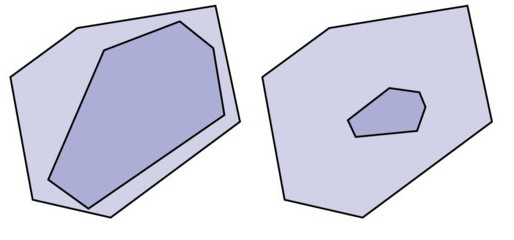
\includegraphics[width=0.1\textwidth]{slike/slide_031.jpg}
\end{center}
	\begin{align*}
		P(\textrm{hit} A | \textrm{hit} B) = \frac{S_A}{S_B}
	\end{align*}
	\begin{itemize}
		\item Surface area heuristic (SAH):
	\end{itemize}
	\begin{align*}
		C = C_{trav} + \frac{S_A}{S_N}N_A C_{isect} + \frac{S_A}{S_N}N_B C_{isect}
	\end{align*}
	Pretpostavke
	\begin{itemize}
		\item Distribucija zraka je nasumična (ne mora vrijediti)
	\end{itemize}
\end{frame}

\begin{frame}{BVH, implementacija}
	\begin{itemize}
		\item Odaberemo nasumičnu os
		\item Sortiramo primitive po toj osi
		\item Pola ih stavimo u jedan pod čvor, pola u drugi
		\item Rekurzivno dijelimo dok svaki primitiv bude u svom \textit{leaf} čvoru
	\end{itemize}
	\begin{center}
		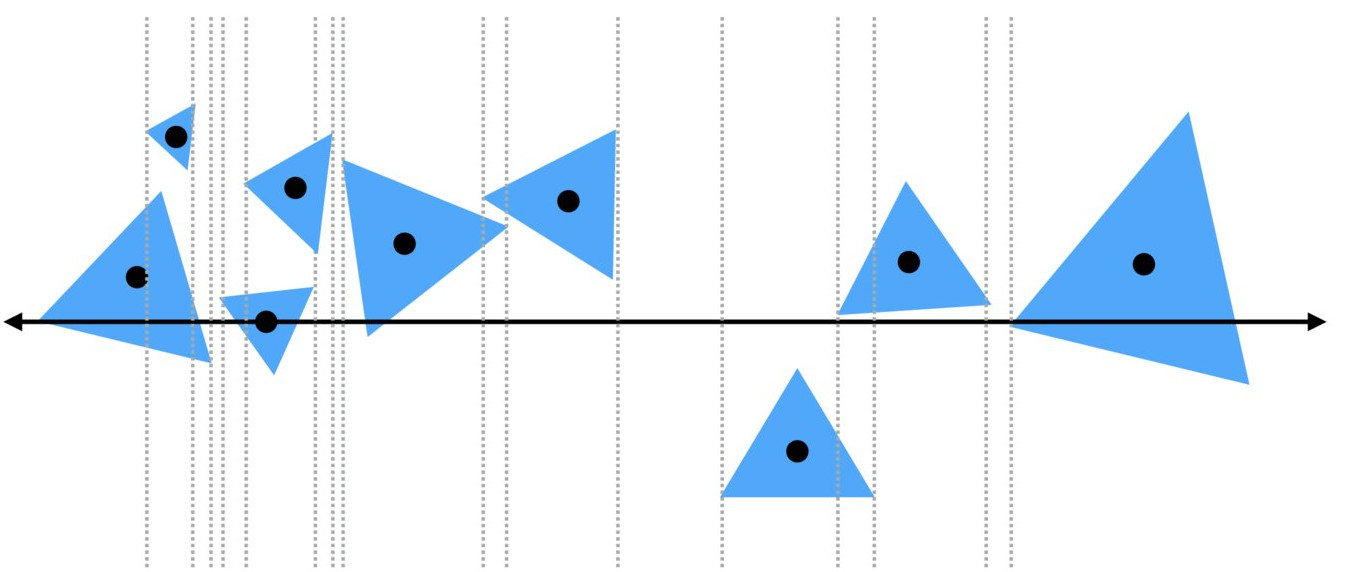
\includegraphics[width=0.8\textwidth]{slike/slide_032.jpg}
	\end{center}
\end{frame}

\begin{frame}{BVH, malo modernijiimplementacija}
	\begin{itemize}
		\item Podijelimo primitite u $B$ segmenata(buckets): $B$ je obično malen: $B<32$
	\end{itemize}
	\begin{center}
		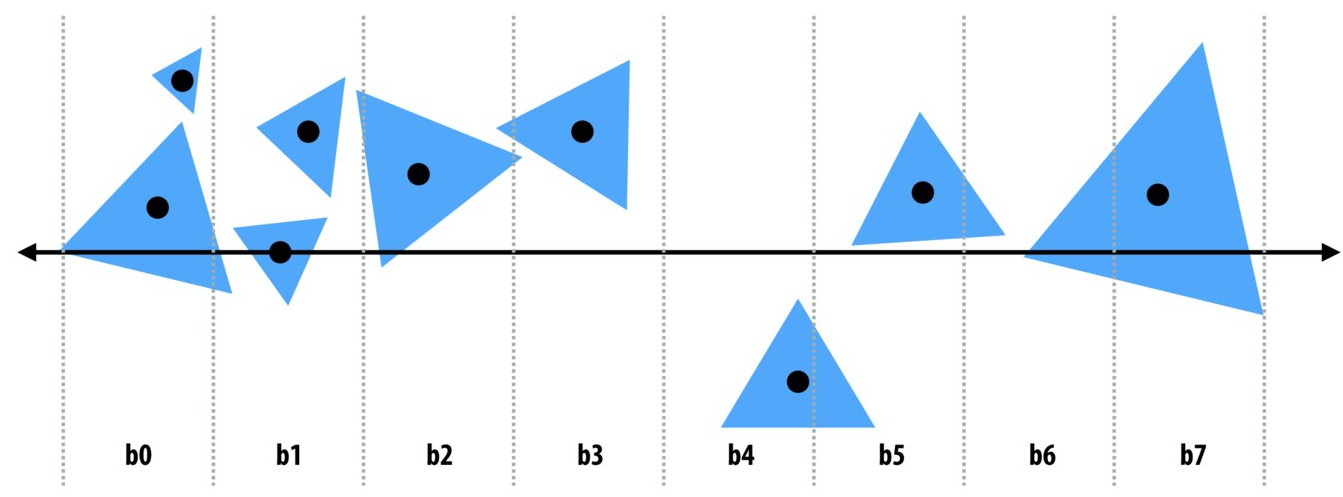
\includegraphics[width=0.8\textwidth]{slike/slide_033.jpg}
	\end{center}
\end{frame}

\begin{frame}{Nije sve idealno}
	\begin{center}
		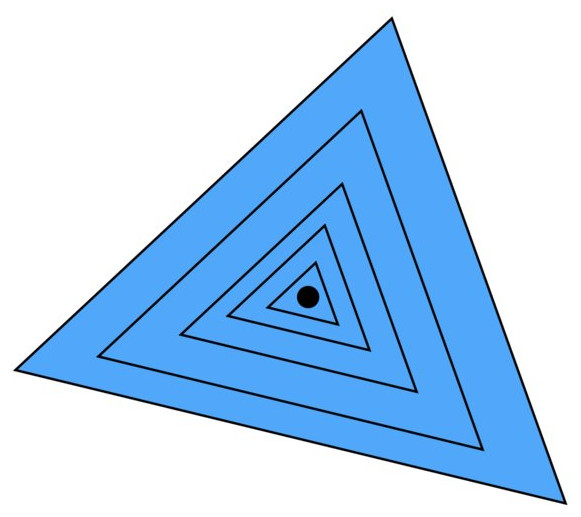
\includegraphics[width=0.2\textwidth]{slike/slide_034_a.jpg}
		\qquad
		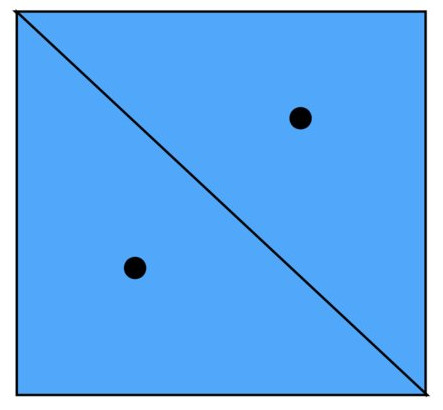
\includegraphics[width=0.2\textwidth]{slike/slide_034_b.jpg}
	\end{center}
\begin{itemize}
	\item Lijevo: Svi primitivi imaju isti centroid
	\item Desno: Primitivi s istim bbox (zraka završi u oba čvora, možda)
\end{itemize}
\end{frame}

\section{Pravokutnik}
\begin{frame}{Primitiv kao izvor svjetla}
	\begin{itemize}
		\item Pravokutnik je definiran u $xy$ ravnini.
		\item Ravnina pravokutnika je definirana $z$ koordinatom, npr. $z=k$
		\item Definiramo još $4$ linije sa $x=x_0$, $x=x_1$, $y=y_0$ i $y=y_1$
	\end{itemize}
	\begin{center}
		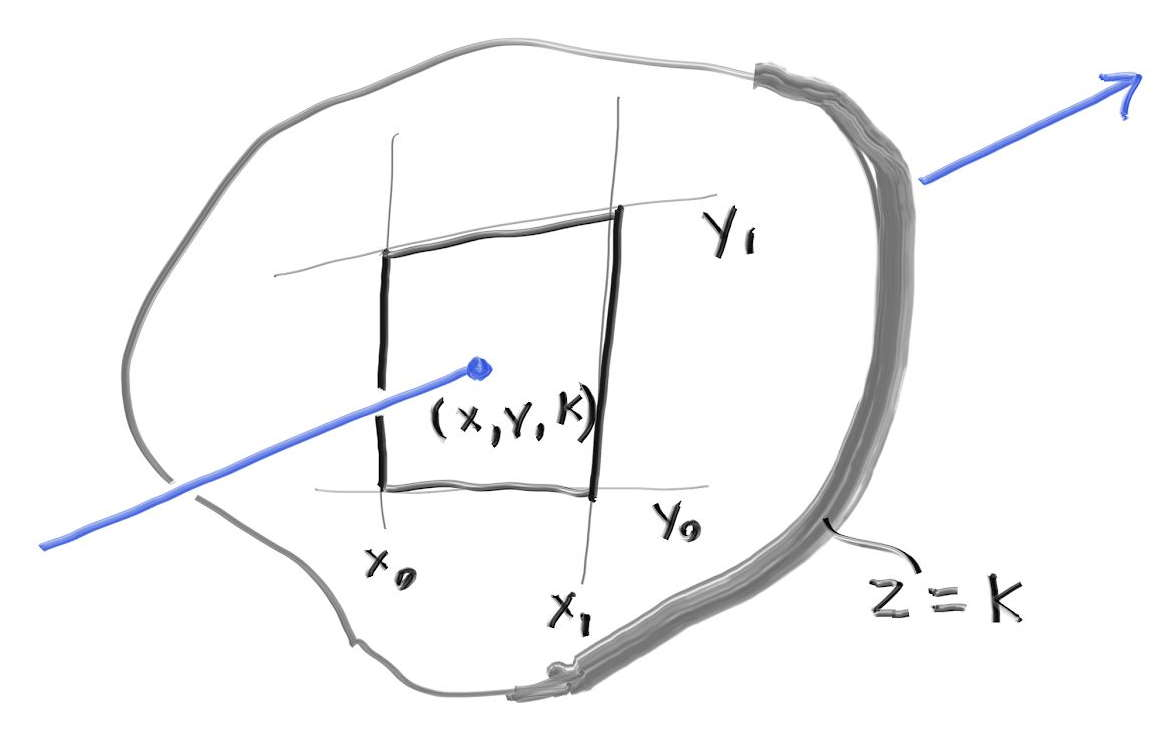
\includegraphics[width=0.2\textwidth]{slike/fig.ray-rect.jpg}
	\end{center}

	Za zraku $\mathbf{P}(t) = \mathbf{o} + t\mathbf{d}$, $z$ komponenta je definirana sa $\mathbf{P}_z(t) = \mathbf{o}_z + t\mathbf{d}_z$. Kako je $z=k$,
	$$
	t = \frac{k-\mathbf{o}_z}{\mathbf{d}_z}
	$$
	Sada možemo izračunati $x$ i $y$:
	\begin{align*}
	x &= \mathbf{o}_x + t\mathbf{d}_x \\
	y &= \mathbf{o}_y + t\mathbf{d}_y \\
	\end{align*}
	Samo još treba provjeriti $x_0 < x < x_1$ i $y_0 < y < y_1$
\end{frame}
\section{Izvori svjetla, emisija}

\begin{frame}{Primitiv kao izvor svjetla}
	\begin{itemize}
		\item Ovo je lako: Ako zraka \textit{udari} u primitiv, postavimo boju svjetla
		\item Zraka se odbija u nasumičnom smjeru, nosi boju svjetla itd...
	\end{itemize}
	\begin{center}
		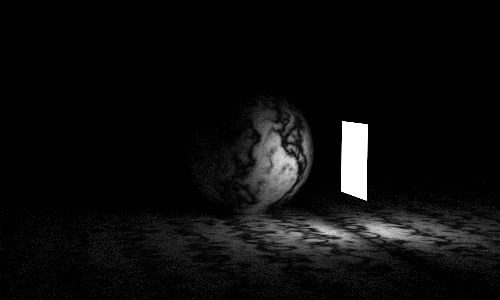
\includegraphics[width=0.6\textwidth]{slike/img.rect-light.jpg}
	\end{center}
\end{frame}


\plain{Pitanja?}
\end{document}